\chapter{Analyse}

\section{Übertragungsmedien}

Somit können als Übertragungsmedien neben der klassischen Kabelverbindung auch andere (instabile) Kanäle wie Mobilfunk oder Satelliten in Frage kommen. Um die Kommunikation über alle Medien sicher und zuverlässig zu gestalten, müssen auf technischer Ebene Protokolle genutzt werden, welche es ermöglichen die gegebenen Schutzziele zu realisieren.

Des Weiteren müssen die Daten über große Entfernungen hinweg übertragen werden. 

\subsection{Kabelgebunden}
\subsection{Funk/instabile Übertragungskanäle}
\subsubsection{\ac{GSM}}
\subsubsection{\ac{HSDPA}}
\subsubsection{\ac{LTE}}
\subsubsection{\ac{LPWA}}

\section{Integrationsansätze}
\subsection{Konsolidierung der Netzwerkkommunikation}
TODO - alles spricht OPC UA

\subsection{Gatewaykommunikation}
TODO - siehe Trumpf, axoom -> Gateways übersetzen von heterogener Netzwerkkommunikation in Protokollstandard für unternehmensübergreifende bzw. externe Kommunikation.
Ansatz: Softwareschwachstellen, Softwarefehler, müssen viele Herstellerprotokolle unterstützen - Probleme?

\subsubsection{Security-Komponenten}
\subsubsection{Router}
\subsubsection{Gateways}

\section{Kommunikationsstack}
\subsection{Physical Layer}
\subsection{Data Link Layer}
\subsection{Network Layer}
\subsection{Transport Layer und End2End Security}
\subsection{Prozess- und Businesslogik - Application Layer}

\section{Protokolle}
\subsection{etablierte Kommunikationsprotokolle}
\subsubsection{HTTP}
\subsubsection{XMPP}
\subsubsection{MQTT}
\subsubsection{CoAP}

\subsection{M2M-Kommunikationsprotokolle}
\subsubsection{OPC UA}
\subsubsection{MTConnect}
\subsection{weitere? PLCOpen, AutomationML}

\section{Probleme bei Migration alter Systeme}
\subsection{Inkompatibilität}
\subsection{spezielle bzw. proprietäre Protokolle}
\subsection{besondere Anforderungen der Shop-Floor-Ebene}
\subsection{Industrial Ethernet}

\section{Angriffsvektoren}
\subsection{Verschlüsselung}
\subsection{Paketversand}
\subsection{TODO}

\section{Maßnahmenkatalog}
\subsubsection{Defense in Depth Strategie - TODO (Kuipers,2006)}
TODO - Beschreibung und Einordnung der Defense in Depth Strategie

\begin{figure}[h]
    \centering
    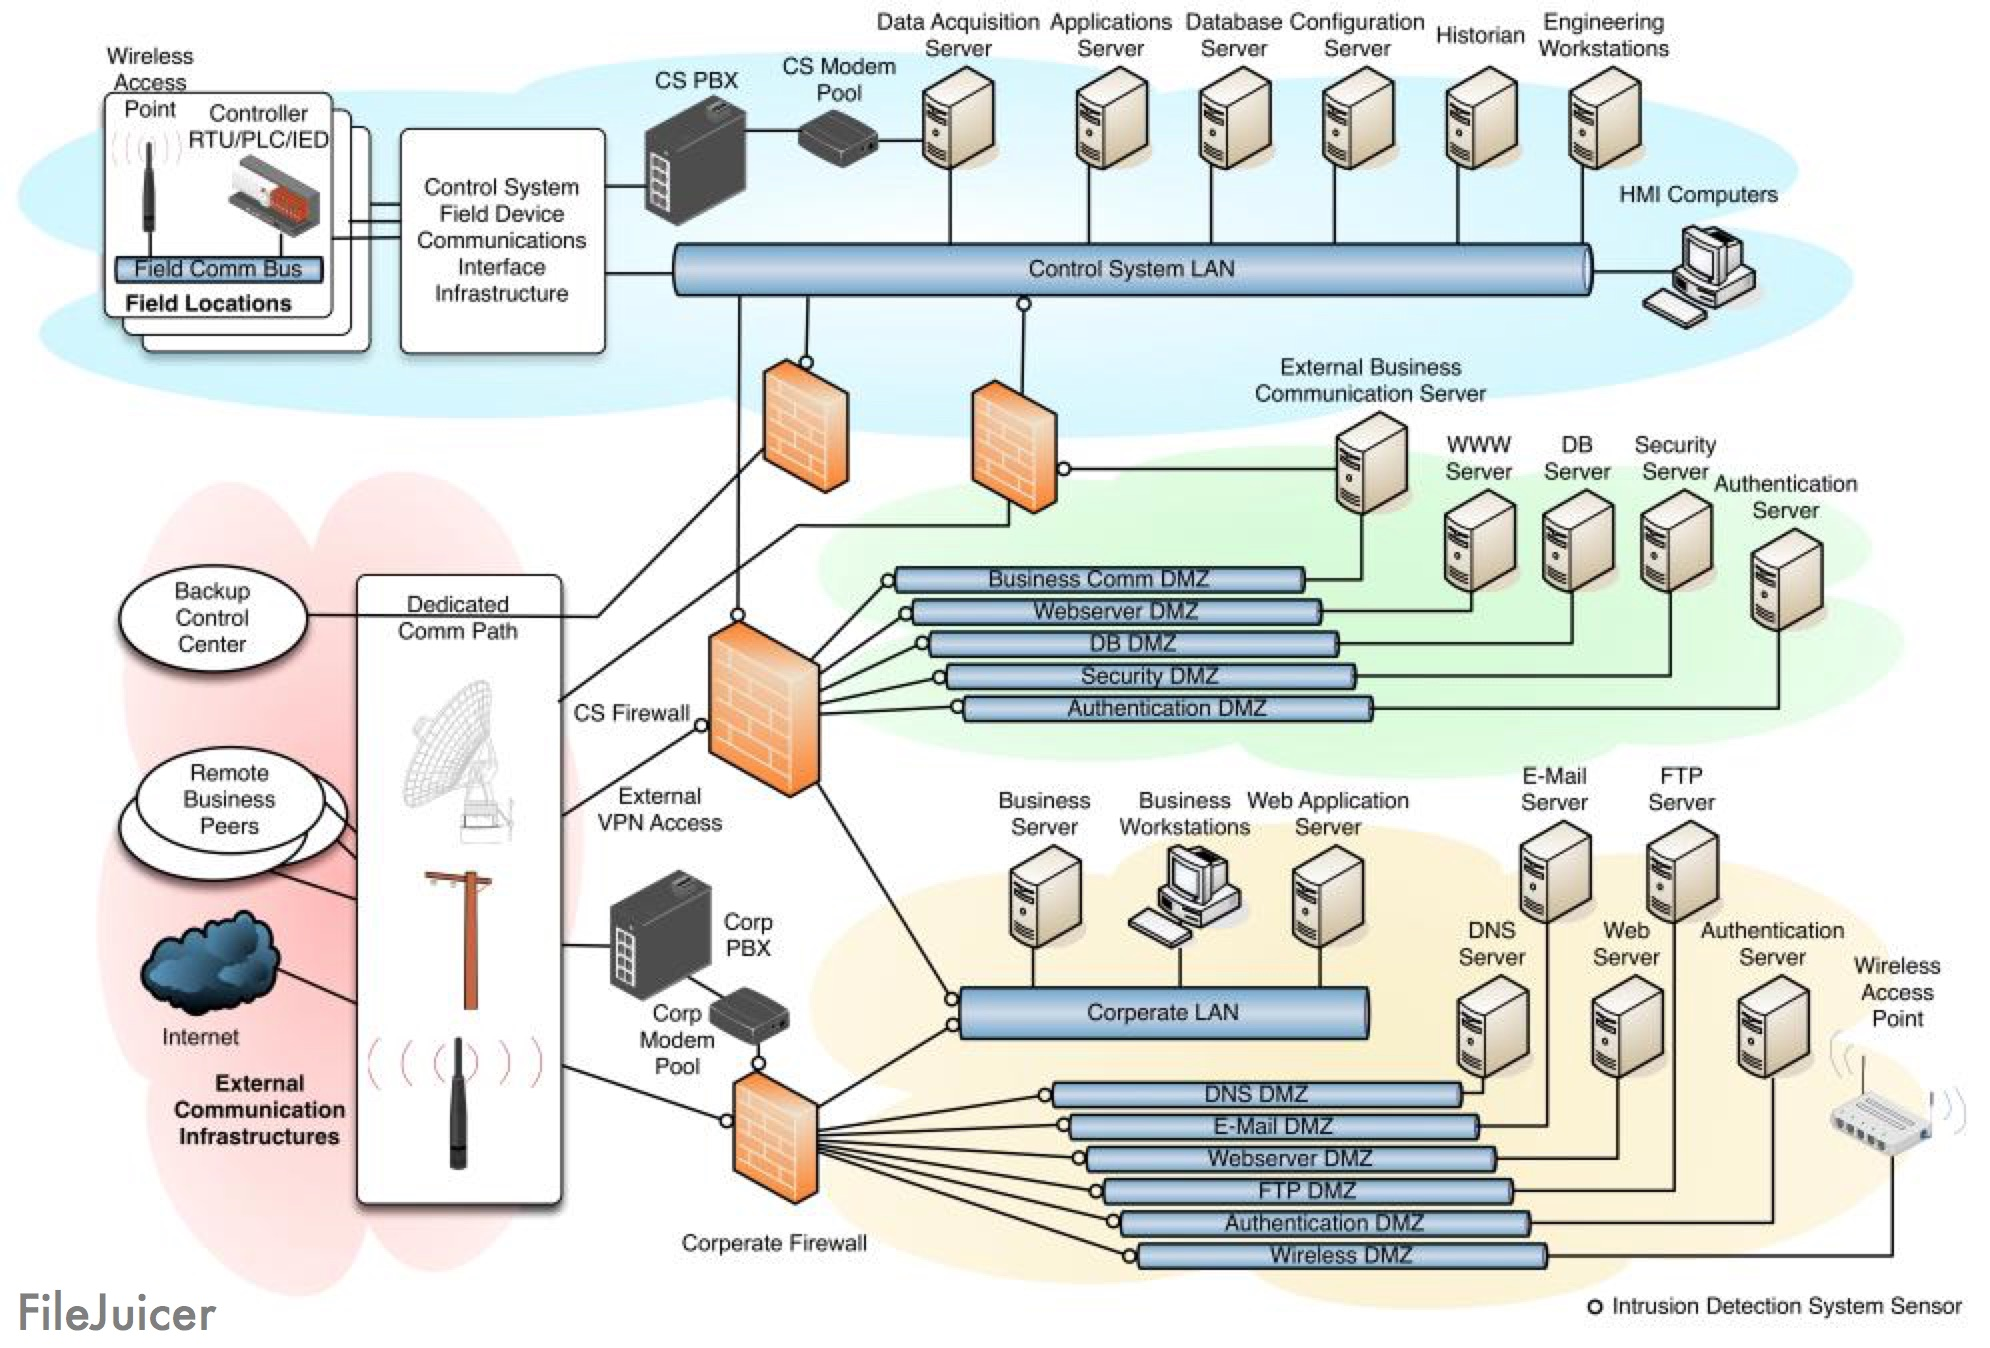
\includegraphics[width=15cm]{defense-in-depth-strategie}
    \caption{Defense in Depth Strategie - TODO ref. Kuipers,2006}
    \label{Kap3:Defense-in-Depth}
\end{figure}